% !TeX program = lualatex
% !TeX encoding = utf8
% !TeX spellcheck = uk_UA

\documentclass[]{beamer}
\usetheme{PlasmaPhysics}
\usepackage{PlasmaPhysics}
\setlength{\abovedisplayskip}{3pt}
\setlength{\belowdisplayskip}{3pt}
\usetikzlibrary{decorations.pathreplacing}
\newtcolorbox{mysidebyside}[1][]{
    notitle, sidebyside, blanker,
    sidebyside align=center seam,
    halign=center,
    lefthand width=.5\textwidth,
    #1
}



\graphicspath{{pictures/}}
\title[Лекції з фізики плазми]{\bfseries\huge Взаємодія електромагнітних хвиль з плазмою}
\subtitle{\bfseries Лекції з фізики плазми}
\author{Пономаренко С. М.}
\date{}
% https://www.youtube.com/watch?v=zv9Y7YmHyBk
\def\stext#1{\text{
        \makebox[0pt]{
            \tikz[baseline] {\node[text width=50pt, align=center, execute at begin node=\setlength{\baselineskip}{-0.5ex}, blue] {#1};}
        }
}}

\setbeamercovered{transparent=25}

%% --------------------------------------------------------
% Радіус Дебая
\NewDocumentCommand{\rD}{}{
    r_D = \sqrt{\frac{T}{4\pi e^2n}}
}

% Плазмова частота
\NewDocumentCommand{\omegap}{}{%
    \omega_p = \sqrt{\frac{4\pi e^2n}{m_e}}
}
%% --------------------------------------------------------

\newcounter{probcnt}
\setcounter{probcnt}{0}

\begin{document}




%===============================================================================
\usebackgroundtemplate{
	\tikz\node[opacity=0.1]{\includegraphics[width=\paperwidth,height=\paperheight]{background}};%
}


\begin{frame}
	\titlepage
\end{frame}

% ============================== Слайд ## ===================================
\begin{frame}{Падіння хвилі на поверхню плазми}{}
	\begin{block}{}
		Нехай на плазму падає плоска електромагнітна хвиля:
		\begin{equation*}
			\vec{E} = E_0 \vec{e}_z e^{-i(\omega t - kx)}.
		\end{equation*}
	\end{block}
	\begin{center}
		\begin{tikzpicture}
    \begin{scope}[shift={(1, 0.3)}]
        \draw[blue, thick, domain=-1.5*pi:0, samples=100] plot (\x, {cos(3*\x r)});
        \draw[blue, thick, domain=0:3, samples=100] plot (\x, {exp(-0.9*\x)*cos(3*\x r)});
        \foreach \x in {-1.45, -1.40, ..., 0}{
        \draw[-latex, red!50] ({pi*\x}, 0) -- ++(0, {cos(3*pi*\x r)});
        }
    \end{scope}
    \begin{scope}
        \foreach \Z in {1,...,1234}
        {
         \pgfmathsetmacro{\Y}{1.5*pi*(0.5*rand)}
         \pgfmathsetmacro{\X}{2*rnd}
         \pgfmathtruncatemacro{\V}{ifthenelse(1*sin(deg(6*\Y))>rand,1,0)}
         \ifnum\V=1
            \fill[ball color=red, draw=none] (\X,\Y) circle (1pt);
         \fi
        }
    \end{scope}
    \begin{scope}[shift={(-1.5*pi, -2)}]
        \draw[-latex] (0, 0) -- ++(1, 0) node[right] {$x$};
        \draw[-latex] (0, 0) -- ++(0, 1) node[left] {$z$};
    \end{scope}
    \begin{scope}[shift={(3,2.1)}]
        \node[circle, ball color=red, inner sep=2pt, font=\scriptsize, text=white] (e) at (0,0) {};
        \node[circle, ball color=blue, inner sep=0, text=white, font=\scriptsize,] (i) at (0,-1) {$+$};
        \draw[-latex, brown, thick, text=black] (e) -- node[right] {$p_z =  -ez$} (i) node[right=5pt, font=\tiny, gray] {Нерухомий іон};
    \end{scope}
\end{tikzpicture}
	\end{center}
	\begin{alertblock}{}\centering
		Іони вважаємо нерухомими.
	\end{alertblock}
\end{frame}
% ===========================================================================

% ============================== Слайд ## ===================================
\begin{frame}{Діелектрична проникність плазми}{}\small
	\begin{block}{Коливання електронів}
		Рівняння руху:
		\begin{equation*}
			\ddot{z} = -\frac{e}{m}E_z
		\end{equation*}
		Розв'язок (закон руху):
		\begin{equation*}
			z = \frac{e}{m\omega^2}E_z
		\end{equation*}
	\end{block}
	\begin{block}{Діелектрична проникність плазми}
		Поляризація плазми:
		\begin{equation*}
			P_z = p_zn = - \frac{e^2}{m\omega^2}E_z = \chi E_z
		\end{equation*}
		Діелектрична проникність:
		\begin{equation*}
			\varepsilon = 1 + 4\pi\chi = 1 - \frac{4\pi e^2 n}{m\omega^2} = 1 - \frac{\omega_p^2}{\omega^2}.
		\end{equation*}
	\end{block}
\end{frame}
% ===========================================================================

% ============================== Слайд ## ===================================
\begin{frame}{Закон дисперсії}{}
	\begin{block}{}
		Для електромагнітної хвилі:
		\begin{equation*}
			k^2 = \left( \frac{\omega}{c}\right)^2\varepsilon =  \left( \frac{\omega}{c}\right)^2\left( 1 - \frac{\omega_p^2}{\omega^2} \right)
		\end{equation*}
		або
		\begin{equation*}
			\omega(k) = \sqrt{\omega_p^2 + c^2k^2}
		\end{equation*}
	\end{block}
	\begin{block}{Фазова швидкість та групова швидкість}
		\begin{align*}
			v_\text{ф}  & = \frac{\omega}{k} = \sqrt{\frac{\omega_p^2}{k^2} + c^2} > c, \quad \text{при}\ k^2 > 0\ (\omega > \omega_p) \\
			v_\text{гр} & = \frac{d\omega}{dk} = \frac{c^2}{\sqrt{\frac{\omega_p^2}{k^2} + c^2}} = \frac{c^2}{v_\text{ф}} < c.
		\end{align*}
	\end{block}
\end{frame}
% ===========================================================================

% ============================== Слайд ## ===================================
\begin{frame}{Закон дисперсії}{}
	\begin{center}
		\begin{tikzpicture}%[scale=0.75, every nodes/.style={transform shape}]
    \begin{axis}[%
%                axis equal,
                scale=.75,
                transform shape,
                every nodes/.style={transform shape},
                xmin=0,
                ymin=0,
    			xlabel=$k$,
    			ylabel=$\omega$,
    			axis lines=middle,
    			every axis x label/.style={at={(current axis.south east)},anchor=north},
    			every axis y label/.style={at={(current axis.north west)}, anchor=east},
%                xticklabel style={font=\scriptsize},
                ytick={sqrt(0.5)},
                yticklabel={$\omega_p$},
    			xtick=\empty,
                legend style={
                at={(current axis.north west)},
                anchor=north west,
                draw=none,
                row sep=0.5ex,
                },
                legend cell align=left,
    			width=\linewidth,
    			height=0.75\linewidth%
    		]
        \addplot[
            blue,
            thick,
            mark=none,
            domain=0:3,
            smooth,
            ] {sqrt(0.5 + x^2)};
            \addlegendentry{$\omega = \sqrt{\omega_p^2 + c^2k^2}$}
        \addplot[
            red,
            thick,
            dashed,
            mark=none,
            domain=0:3,
            smooth,
            ] {x};
            \addlegendentry{$\omega = ck$}
    \end{axis}
\end{tikzpicture}
	\end{center}
\end{frame}
% ===========================================================================

% ============================== Слайд ## ===================================
\begin{frame}{Падіння хвилі на діелектрик}{}
	\begin{columns}
		\begin{column}{0.5\linewidth}
			\begin{center}
				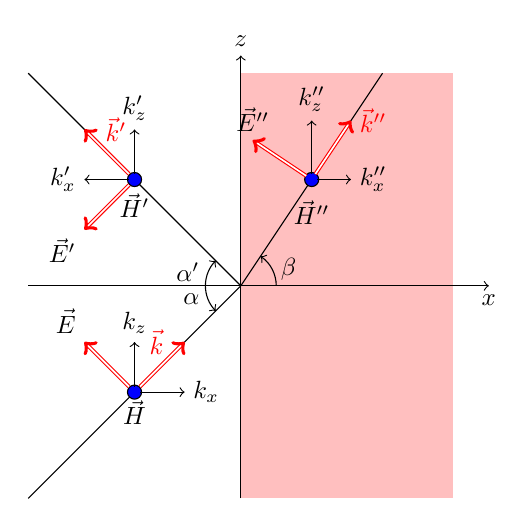
\begin{tikzpicture}[scale=0.9, every node/.style={transform shape}]
	\fill[red!50, opacity=0.5] (0, -3) rectangle (3, 3);
	\draw[->] (0, -3) to (0,3.25) node[above] {$z$};
	\draw[->] (-3, 0) to (3.5,0) node[below] {$x$};
	%        \node[circle, draw, anchor=north west, fill=cyan, font=\scriptsize, inner sep=1pt] at (-1, 3) {1};
	%        \node[circle, draw, anchor=north west, fill=cyan, font=\scriptsize, inner sep=1pt] at (1, 3) {2};
	\draw (-3, -3) -- node[pos = 0.5, inner sep=2pt] (A) {} (0, 0) ;
	\node[circle, draw, inner sep=2pt, fill=blue] at (A) {};
	\node[below] at (A) {$\vec{H}$};
	\draw[->, red, double] (A) -- ++(45:1) node[left=5pt] {$\vec{k}$};
	\draw[->] (-0.5, 0) arc (180:225:0.5) node[left, pos=0.5] {$\alpha$};
	\draw[->] (A) -- ++(0:{cos(45)}) node[right] {$k_x$};
	\draw[->] (A) -- ++(90:{sin(45)}) node[above] {$k_z$};
	\draw[red, ->, double, text=black] (A) -- ++(({atan(3/3) + 90}:1) node[above left] {$\vec{E}$};

	\draw (0, 0) -- node[pos = 0.5, inner sep=2pt] (B) {} (-3, 3);
	\node[circle, draw, inner sep=2pt, fill=blue] at (B) {};
	\node[below=2pt] at (B) {$\vec{H}'$};
	\draw[->, red, double] (B) -- ++(135:1) node[right=5pt] {$\vec{k}'$};
	\draw[->] (-0.5, 0) arc (180:135:0.5) node[left, pos=0.5] {$\alpha'$};
	\draw[->] (B) -- ++(0:-{cos(45)}) node[left] {$k'_x$};
	\draw[->] (B) -- ++(90:{sin(45)}) node[above] {$k'_z$};
	\draw[red, ->, double, text=black] (B) -- ++(({-atan(3/3) - 90}:1) node[below left] {$\vec{E}'$};

	\pgfmathsetmacro{\angle}{atan(3/2)}
	\draw (0, 0) -- node[pos = 0.5, inner sep=2pt] (C) {} (2, 3);
	\node[circle, draw, inner sep=2pt, fill=blue] at (C) {};
	\node[below=5pt] at (C) {$\vec{H}''$};
	\draw[->, red, double] (C) -- ++({atan(3/2)}:1) node[right] {$\vec{k}''$};
	\draw[->] (0.5, 0) arc (0:\angle:0.5) node[right, pos=0.5] {$\beta$};
	\draw[->] (C) -- ++(0:{cos{\angle}}) node[right] {$k''_x$};
	\draw[->] (C) -- ++(90:{sin(\angle)}) node[above] {$k''_z$};
	\draw[red, ->, double, text=black] (C) -- ++(({\angle + 90}:1) node[above] {$\vec{E}''$};
\end{tikzpicture}
			\end{center}
		\end{column}
		\begin{column}{0.5\linewidth}
			\begin{block}{}\scriptsize
				Граничні умови $H_{\tau_1} = H_{\tau_2}$ та $E_{\tau_1} = E_{\tau_2}$ дають:
				\begin{equation*}
					H_0 + H'_0 = H''_0 \Rightarrow E_0 + E'_0 = \sqrt{\varepsilon} E''_0
				\end{equation*}
				\begin{equation*}
					E_0\cos\alpha - E'_0\cos\alpha = E''_0 \cos\beta.
				\end{equation*}
				З цих умов випливає:
				\begin{equation*}
					E'_0 = \frac{\sqrt{\varepsilon}\ \cos \alpha - \cos\beta}{\sqrt{\varepsilon}\ \cos\alpha + \cos\beta} E_0
				\end{equation*}
				Коефіцієнт відбивання:
				\begin{equation*}
					R = \left|\frac{E'_0}{E_0}\right|^2 = \left|\frac{1 - \dfrac1{\sqrt{\varepsilon}} \dfrac{\cos \beta}{\cos \alpha} }{1 + \dfrac1{\sqrt{\varepsilon}} \dfrac{\cos \beta}{\cos \alpha}}\right|^2
				\end{equation*}
				Закон заломлення:
				\begin{equation*}
					\sin\alpha = \sqrt\varepsilon\sin\beta.
				\end{equation*}
			\end{block}
		\end{column}
	\end{columns}

\end{frame}
% ===========================================================================

% ============================== Слайд ## ===================================
\begin{frame}{Випадок $ \omega < \omega_p$ ($\varepsilon < 0$)}{}
	\begin{block}{}\small\justifying
		Показник заломлення стає суто уявною величиною
		\begin{equation*}
			\sqrt{\varepsilon} = i\chi
		\end{equation*}
		Коефіцієнт відбивання хвилі:
		\begin{equation*}
			R = \left|\frac{1 + i\chi \dfrac{\cos \beta}{\cos \alpha} }{1 - i\chi \dfrac{\cos \beta}{\cos \alpha}}\right|^2 = 1
		\end{equation*}
		Хвильове число:
		\begin{equation*}
			k = \frac{\omega}{c}\sqrt{\varepsilon} = i \frac{\omega}{c}\chi = i\kappa.
		\end{equation*}
		Електричне поле $\vec{E}''$ в плазмі:
		\begin{equation*}
			\vec{E}'' = \vec{e}_z E''_0  e^{-i(\omega t - kx)} = \vec{e}_z E''_0e^{-\kappa x}  e^{-i\omega t}.
		\end{equation*}
		Це означає, що амплітуда хвилі експоненціально спадає --- хвиля
		загасає при заглибленні в плазму.
	\end{block}
\end{frame}
% ===========================================================================

% ============================== Слайд ## ===================================
\begin{frame}{Зондування плазми}
	\framesubtitle<1>{Мікрохвильове зондування}
	\framesubtitle<2>{Мікрохвильовий інтерферометр}
	\begin{overprint}
		\onslide<1>
		\begin{center}
			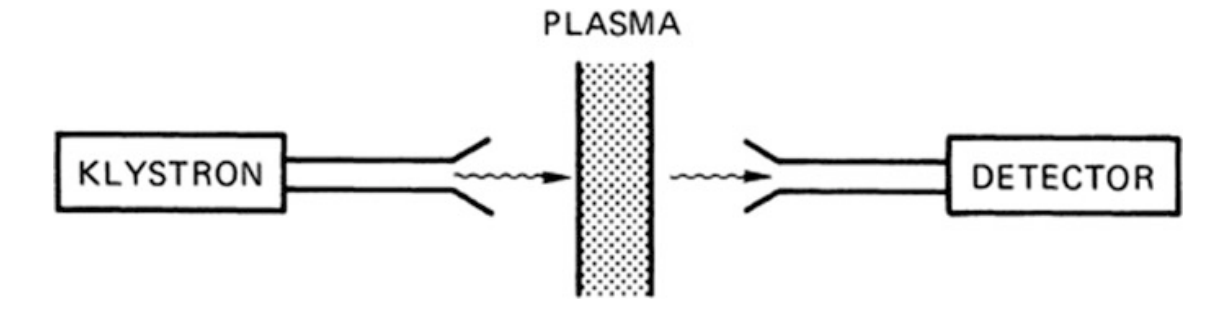
\includegraphics[width=0.85\linewidth]{plasma_zond}
		\end{center}
		\begin{block}{}\small\justifying
			Плазму просвічують спрямованим пучком електромагнітних хвиль. Якщо хвиля проходить через плазму і детектується приймачем, поміщеним з іншого боку, то концентрація плазми нижча за граничну. <<Запирання>> (cutoff) електромагнітного сигналу означає, що концентрація плазми вища за граничну.

			\medskip

			{\scriptsize  Для часто вживаних хвиль з довжиною $3$~см гранична концентрація становить $10^{12}$~см\textsuperscript{-3}.     Поширення хвиль можна спостерігати тільки за умови достатнього віддалення від випромінювача, у так званій хвильовій зоні.
			}

		\end{block}
		\onslide<2>
		\begin{center}
			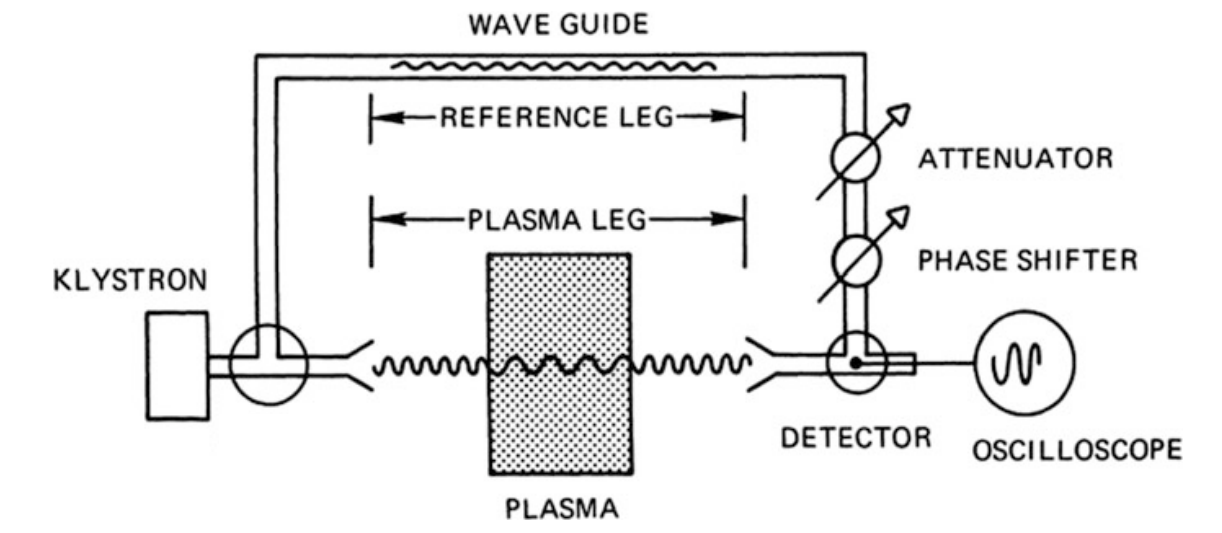
\includegraphics[width=0.85\linewidth]{plasma_interferometry}
		\end{center}
		\begin{block}{}\small\justifying
			Спрямований радіосигнал із частотою, вищою за плазмову, ділиться на два промені. Один пропускається через плазму, інший --- через середовище з показником заломлення $ n = 1 $ (повітря). Через відмінності у фазових швидкостях у променів виникає різниця у фазах, яку вимірюють інтерферометром.

			\medskip

			{\scriptsize Цим методом визначають фактично фазову швидкість електромагнітної хвилі в плазмі, яка через дисперсію залежить від концентрації.}
		\end{block}
	\end{overprint}
\end{frame}
% ===========================================================================

% ============================== Слайд ## ===================================
\begin{frame}{Принципи дальнього зв'язку на УКХ}{}

	\begin{overprint}
		\onslide<1>
		\begin{block}{}\justifying\small
			Іоносфера --- шари атмосфери на висоті від $80$ до $600$~км, які характеризуються високим вмістом іонів і вільних електронів. Іонізація відбувається під впливом ультрафіолетових променів сонячної радіації. Складається зі суміші газу нейтральних атомів і молекул (переважно азот \ce{N2} і кисень \ce{O2}) і плазми.
		\end{block}
		\onslide<2>
		\begin{block}{}\justifying\small
			Шар F (від $150 \div 600$~км відбиває радіохвилі в діапазоні коротких хвиль на частотах від декількох мегагерц до $10$ МГц, що робить можливим передавання таких радіосигналів на значні відстані (Едвард Віктор Еплтон, Нобелівська премія з фізики 1947 року.)
		\end{block}
	\end{overprint}
	\begin{center}
		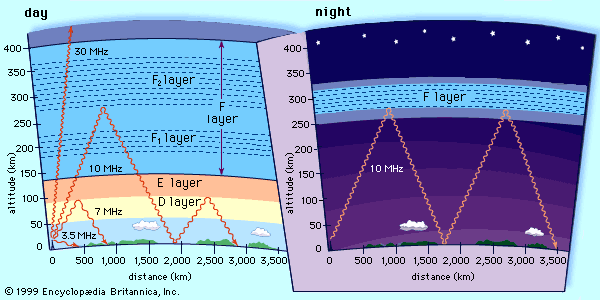
\includegraphics[width=0.9\linewidth]{ionosphere}
	\end{center}


\end{frame}
% ===========================================================================

% ============================== Слайд ## ===================================
\begin{frame}{Задачі}{}


	\begin{onlyenv}<1>
		\begin{exampleblock}{\scriptsize\color{blue} Задача 1}\scriptsize\justifying
			Під час зондування розрідженої плазми радіохвилями різних частот установлено, що радіохвилі з частотами, меншими за $400$ МГц, не проходять крізь плазму. Знайти концентрацію вільних електронів у плазмі  $N_e$.% = 2.0⋅10^9$~ см\textsuperscript{-3}.
		\end{exampleblock}

		\begin{exampleblock}{\scriptsize\color{blue} Задача 2}\scriptsize\justifying% Козел 4.116
			Показник заломлення іоносфери для радіохвиль із частотою $ \nu= 10$~МГц дорівнює $n = 0.90$. Знайти концентрацію $N$ електронів в іоносфері, а також фазову і групову швидкості для цих радіохвиль.
		\end{exampleblock}

		\begin{exampleblock}{\scriptsize\color{blue} Задача 3}\scriptsize\justifying% Козел 4.117
			Під час вивчення проходження плоскої електромагнітної хвилі частотою $\nu = 8$~МГц через плоскі однорідні шари плазми з концентрацією вільних електронів $N = 10^6 $~см\tsup{-3} знайдено, що енергетичні коефіцієнти пропускання хвиль різняться в $10$ разів для шарів плазми, товщина яких різниться вдвічі. Нехтуючи інтенсивністю хвиль, відбитих від задньої межі кожного шару, знайти їхні товщин.
		\end{exampleblock}


		\begin{exampleblock}{\scriptsize\color{blue} Задача 4}\scriptsize\justifying% Козел 4.122
			Визначити число вільних електронів на атом \ce{Ag}, якщо плівка срібла прозора для ультрафіолету, починаючи з енергії $W = 5$~еВ. Для срібла відносна атомна маса дорівнює $A = 108$, густина $\rho = 10.5$~г/см\tsup{3}.
		\end{exampleblock}
	\end{onlyenv}

	\begin{onlyenv}<2>

		\begin{exampleblock}{\scriptsize\color{blue} Задача 5}\scriptsize\justifying% Козел 4.119
			Імпульсне випромінювання пульсара \href{https://en.wikipedia.org/wiki/PSR\_B1919\%2B21}{\color{blue} PSR B1919+21} на частоті $\nu_1 =80 $ МГц досягає Землі на $\Delta t = 7$~с пізніше, ніж відповідний імпульс на частоті $\nu_2 = 2000 $~МГц. Оцінити відстань до пульсара, якщо прийняти середню концентрацію електронів у міжзоряному просторі рівною $0.05$~см\tsup{-3}.
		\end{exampleblock}
		\begin{exampleblock}{\scriptsize\color{blue} Задача 6}\scriptsize\justifying% Козел 4.118
			Для оцінювання інтегральних і середніх характеристик міжзоряної плазми можна використати експериментальний факт, установлений одразу ж після відкриття пульсарів. Виявилося, що через дисперсію плазми імпульси радіовипромінювання пульсарів на нижчих частотах завжди запізнюються щодо імпульсів вищих частот. Розгляньте наступ\-ний ідеалізований приклад. Два монохроматичні сигнали з довжинами хвиль $\lambda = 3$~см і $\lambda = 5$~см поширюються в плазмі. Визначити повне число $N$ вільних електронів на шляху сигналів (тобто їхнє число в циліндрі площею $1$~см\tsup{2} і висотою, що дорівнює відстані джерело-приймач), якщо випущені одночасно сигнали запізнюються відносно один одного на час $\Delta t = 10^{-5}$~с. Концентрація електронів хоча й не постійна вздовж шляху сигналів, але показник заломлення скрізь дуже близький до одиниці. Визначити також середню концентрацію $n$ вільних електронів на шляху сигналів, якщо їхнє відносне запізнювання $\Delta t/t_0 = 10^{-15}$ ($t_0$ --- час поширення від джерела до приймача).
		\end{exampleblock}
	\end{onlyenv}
\end{frame}
% ===========================================================================

\end{document}

